\documentclass[a4paper,11pt]{article}
\usepackage[polish]{babel}
\usepackage[utf8]{inputenc}   % lub utf8
\usepackage[T1]{fontenc}
\usepackage{graphicx}
\usepackage{anysize}
\usepackage{enumerate}
\usepackage{times}
\usepackage{tikz}
%\marginsize{left}{right}{top}{bottom}
\marginsize{3cm}{3cm}{3cm}{3cm}

\sloppy

\begin{document}
\begin{figure}
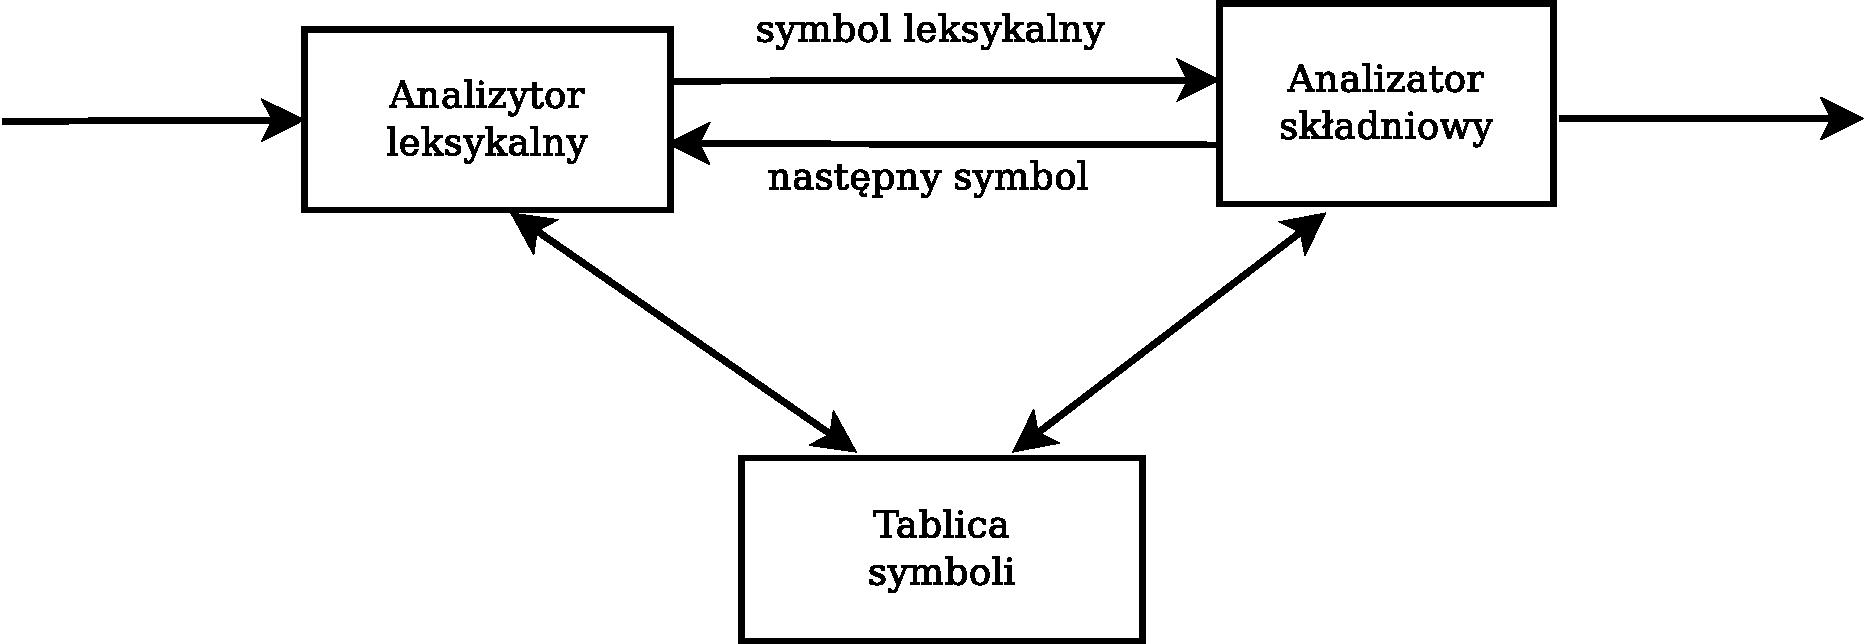
\includegraphics[scale=0.5]{diag.pdf}
\caption{diagram}
\label{fig:diagram}
\end{figure}

\begin{figure}[!htb]
\centering
\begin{tikzpicture}
	\node at(0,0) {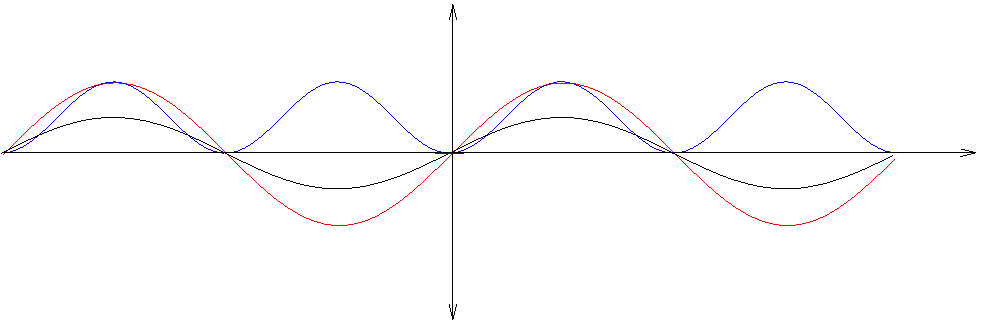
\includegraphics[scale=1]{f1.pdf}};
	\node at(5.6,-1.5) {$f(x) = \sin(x)$};
	\node at(1,0.4) {$h(x) = \frac{\sin(x)}{2}$};
	\node at(5.5,1.6) {$g(x) = sin^2(x)$};
\end{tikzpicture}
\caption{wykres}
\label{fig:wykres}
\end{figure}
\end{document}